
\section{Luminosity Function}\label{app: lum_func}
\begin{table*}
	\centering
	\begin{tabular}[t]{cccccc}
		\hline
		M$_{1500}$ &  $\phi$\,/(cMpc$^{-3}$ Mag$^{-1}$) & M$_{1500}$ &  $\phi$\,/(cMpc$^{-3}$ Mag$^{-1}$) & M$_{1500}$ &  $\phi$\,/(cMpc$^{-3}$ Mag$^{-1}$)\\
		\hline
		\multicolumn{2}{c}{z = 5} & \multicolumn{2}{c}{z = 6} & \multicolumn{2}{c}{z = 7} \\
		\hline
		-24.245 &  (3.620$\pm$3.620)$\times 10^{-8}$ & -23.767 &  (1.473$\pm$1.473)$\times 10^{-9}$ & -23.508 &  (1.473$\pm$1.473)$\times 10^{-9}$ \\
		-23.745 &  (3.261$\pm$1.295)$\times 10^{-7}$ & -23.267 &  (3.787$\pm$1.329)$\times 10^{-7}$ & -23.008 &  (1.505$\pm$  0.828)$\times 10^{-7}$ \\
		-23.245 &  (2.218$\pm$1.596)$\times 10^{-6}$ & -22.767 &  (9.617$\pm$3.048)$\times 10^{-7}$ & -22.508 &  (9.128$\pm$3.036)$\times 10^{-7}$ \\
		-22.745 & (6.507$\pm$3.423)$\times 10^{-6}$ & -22.267 &  (7.815$\pm$2.459)$\times 10^{-6}$ & -22.008 &  4.498$\pm$2.214)$\times 10^{-6}$ \\
		-22.245 &  (2.817$\pm$0.668)$\times 10^{-5}$ & -21.767 &  (2.692$\pm$0.690)$\times 10^{-5}$ & -21.508 &  (1.939$\pm$0.605)$\times 10^{-5}$ \\
		-21.745 &  (6.530$\pm$1.155)$\times 10^{-5}$ & -21.267 &  (8.620$\pm$1.378)$\times 10^{-5}$ & -21.008 &  (4.658$\pm$1.003)$\times 10^{-5}$ \\
		-21.245 &  (1.569$\pm$0.187)$\times 10^{-4}$ & -20.767 &  (1.718$\pm$0.204)$\times 10^{-4}$ & -20.508 &  (9.793$\pm$1.491)$\times 10^{-5}$ \\
		-20.745 &  (4.672$\pm$0.350)$\times 10^{-4}$ & -20.267 &  (3.299$\pm$0.293)$\times 10^{-4}$ & -20.008 &  (2.532$\pm$0.257)$\times 10^{-4}$ \\
		-20.245 &  (6.789$\pm$0.425)$\times 10^{-4}$ & -19.767 &  (5.165$\pm$0.364)$\times 10^{-4}$ & -19.508 &  (4.075$\pm$0.330)$\times 10^{-4}$ \\
		-19.745 &  (9.953$\pm$0.527)$\times 10^{-4}$ & -19.267 &  (9.396$\pm$0.514)$\times 10^{-4}$ & -19.008 &  (6.639$\pm$0.415)$\times 10^{-4}$ \\
		-19.245 &  (1.566$\pm$0.066)$\times 10^{-3}$ & -18.767 &  (1.697$\pm$0.070)$\times 10^{-3}$ & -18.508 &  (1.755$\pm$0.070)$\times 10^{-3}$ \\
		-18.745 &  (2.571$\pm$0.086)$\times 10^{-3}$ & -18.267 &  (3.431$\pm$0.010)$\times 10^{-3}$ & -18.008 &  (3.897$\pm$0.107)$\times 10^{-3}$ \\
		-18.245 &  (4.478$\pm$0.115)$\times 10^{-3}$ & -17.767 &  (6.178$\pm$0.135)$\times 10^{-3}$ & -17.508 &  (6.404$\pm$0.138)$\times 10^{-3}$ \\
		-17.745 &  (7.719$\pm$0.152)$\times 10^{-3}$ & -17.267 &  (9.171$\pm$0.166)$\times 10^{-3}$ &   -- &  --  \\
		-17.245 &  (1.105$\pm$0.018)$\times 10^{-2}$ &   -- &  -- &  -- &   -- \\
		\hline
	\end{tabular}
	\begin{tabular}[t]{cccccc}
		\hline
		M$_{1500}$ &  $\phi$\,/(cMpc$^{-3}$ Mag$^{-1}$) & M$_{1500}$ &  $\phi$\,/(cMpc$^{-3}$ Mag$^{-1}$) & M$_{1500}$ &  $\phi$\,/(cMpc$^{-3}$ Mag$^{-1}$)\\
		\hline
		\multicolumn{2}{c}{z = 8} & \multicolumn{2}{c}{z = 9} & \multicolumn{2}{c}{z = 10} \\
		\hline
		-22.682 &  (2.407$\pm$2.407)$\times 10^{-8}$ & -22.605 &  (2.407$\pm$2.407)$\times 10^{-8}$ & -22.513 &  (2.407$\pm$2.407)$\times 10^{-8}$ \\
		-22.182 &  (2.403$\pm$1.544)$\times 10^{-6}$ & -22.105 &  (2.183$\pm$0.872)$\times 10^{-7}$ & -21.513 &  (6.303$\pm$4.580)$\times 10^{-8}$ \\
		-21.682 &  (1.451$\pm$0.307)$\times 10^{-6}$ & -21.605 &  (2.588$\pm$1.621)$\times 10^{-6}$ & -21.013 &  (9.384$\pm$3.790)$\times 10^{-7}$ \\
		-21.182 &  (1.291$\pm$0.448)$\times 10^{-5}$ & -21.105 &  (1.291$\pm$0.375)$\times 10^{-6}$ & -20.513 &  (1.084$\pm$0.454)$\times 10^{-5}$ \\
		-20.682 &  (4.464$\pm$1.026)$\times 10^{-5}$ & -20.605 &  (2.496$\pm$0.764)$\times 10^{-5}$ & -20.013 &  (1.242$\pm$0.397)$\times 10^{-5}$ \\
		-20.182 &  (7.106$\pm$1.310)$\times 10^{-5}$ & -20.105 &  (4.122$\pm$1.009)$\times 10^{-5}$ & -19.513 &  (5.268$\pm$1.098)$\times 10^{-5}$ \\
		-19.682 &  (1.429$\pm$0.1917)$\times 10^{-4}$ & -19.605 &  (8.132$\pm$1.352)$\times 10^{-5}$ & -19.013 &  (1.921$\pm$0.225)$\times 10^{-4}$ \\
		-19.182 &  (3.406$\pm$0.301)$\times 10^{-4}$ & -19.105 &  (2.312$\pm$0.250)$\times 10^{-4}$ & -18.513 &  (5.412$\pm$0.386)$\times 10^{-4}$ \\
		-18.682 &  (8.836$\pm$0.495)$\times 10^{-4}$ & -18.605 &  (7.337$\pm$0.451)$\times 10^{-4}$ & -18.013 &  (1.443$\pm$0.064)$\times 10^{-3}$ \\
		-18.182 &  (2.201$\pm$0.079)$\times 10^{-3}$ & -18.105 &  (1.857$\pm$0.073)$\times 10^{-3}$ &   -- &  -- \\
		-17.682 &  (3.856$\pm$0.105)$\times 10^{-3}$ & -17.605 &  (3.029$\pm$0.094)$\times 10^{-3}$ &   -- &  -- \\
		\hline
	\end{tabular}
	\caption{Binned UVLF values for the \flares\, galaxies. \label{tab: LF values}}
\end{table*}
\begin{table*}
	\centering
	\begin{tabular}[t]{cccccc}
		\hline
		z &  M$^{*}$/Mag &  log$_{10}$($\phi^{*}$\,/(Mpc$^{-3}$ Mag$^{-1}$)) &  $\alpha$ & $\beta$ & $\Delta$BIC\\
		\hline\\
		& -21.812$^{+0.040}_{-0.040}$ & -3.674$^{+0.024}_{-0.025}$ &  -1.987$^{+0.006}_{-0.006}$ & --\\5&&&&& -42.807\\
		& -21.658$^{+0.036}_{-0.036}$ & -3.771$^{+0.022}_{-0.022}$ & -2.034$^{+0.006}_{-0.006}$ & -4.306$^{+0.084}_{-0.095}$\\\\
		& -21.484$^{+0.030}_{-0.028}$ &  -3.869$^{+0.021}_{-0.020}$ &  -2.141$^{+0.007}_{-0.007}$ & --\\6&&&&&97.627\\
		& -21.446$^{+0.026}_{-0.026}$ & -4.054$^{+0.018}_{-0.018}$ & -2.218$^{+0.006}_{-0.006}$ & -5.194$^{+0.009}_{-0.004}$\\\\
		& -21.465$^{+0.040}_{-0.036}$ &  -4.353$^{+0.033}_{-0.031}$ &  -2.421$^{+0.010}_{-0.010}$ & --\\7&&&&& 29.466\\
		& -21.380$^{+0.041}_{-0.040}$ & -4.500$^{+0.032}_{-0.041}$ & -2.500$^{+0.009}_{-0.009}$ & -5.190$^{+0.016}_{-0.008}$\\\\
		& -20.946$^{+0.088}_{-0.086}$ &  -4.379$^{+0.076}_{-0.075}$ &  -2.584$^{+0.019}_{-0.018}$ & --\\8&&&&& 23.969\\
		& -20.966$^{+0.605}_{-0.160}$ & -4.605$^{+0.518}_{-0.136}$ & -2.674$^{+0.097}_{-0.025}$ & -4.773$^{+0.632}_{-0.332}$\\\\
		& -20.458$^{+0.005}_{-0.013}$ &  -4.299$^{+0.015}_{-0.017}$ &  -2.671$^{+0.013}_{-0.013}$ & --\\9&&&&& -79.294\\
		& -19.712$^{+0.009}_{-0.020}$ & -3.812$^{+0.014}_{-0.020}$ & -2.567$^{+0.016}_{-0.016}$ & -4.467$^{+0.079}_{-0.086}$\\\\
		& -20.084$^{+0.123}_{-0.177}$ & -4.416$^{+0.142}_{-0.203}$ &  -3.053$^{+0.050}_{-0.058}$ & --\\10&&&&& -2.676\\
		& -19.658$^{+0.112}_{-0.180}$ & -4.148$^{+0.125}_{-0.204}$ & -3.008$^{+0.057}_{-0.074}$ & -4.864$^{+0.166}_{-0.182}$\\\\
		\hline
	\end{tabular}
	\caption{Best-fitting Schechter (first row corresponding to the redshift) and double power-law (second row corresponding to the redshift) function parameter values for the observed UVLF. In case of the Schechter fit as well as the double power-law fit for $z=9, 10$ we implement narrow priors to M$^*$ which was set by visual inspection in order to constrain the fit. We also provide the difference of the Bayesian Information Criterion ($\Delta$BIC) value of the best-fitting parameters of the Schechter from the double power-law function. \label{tab: fit params}}
\end{table*}
\begin{figure*}
	\centering
	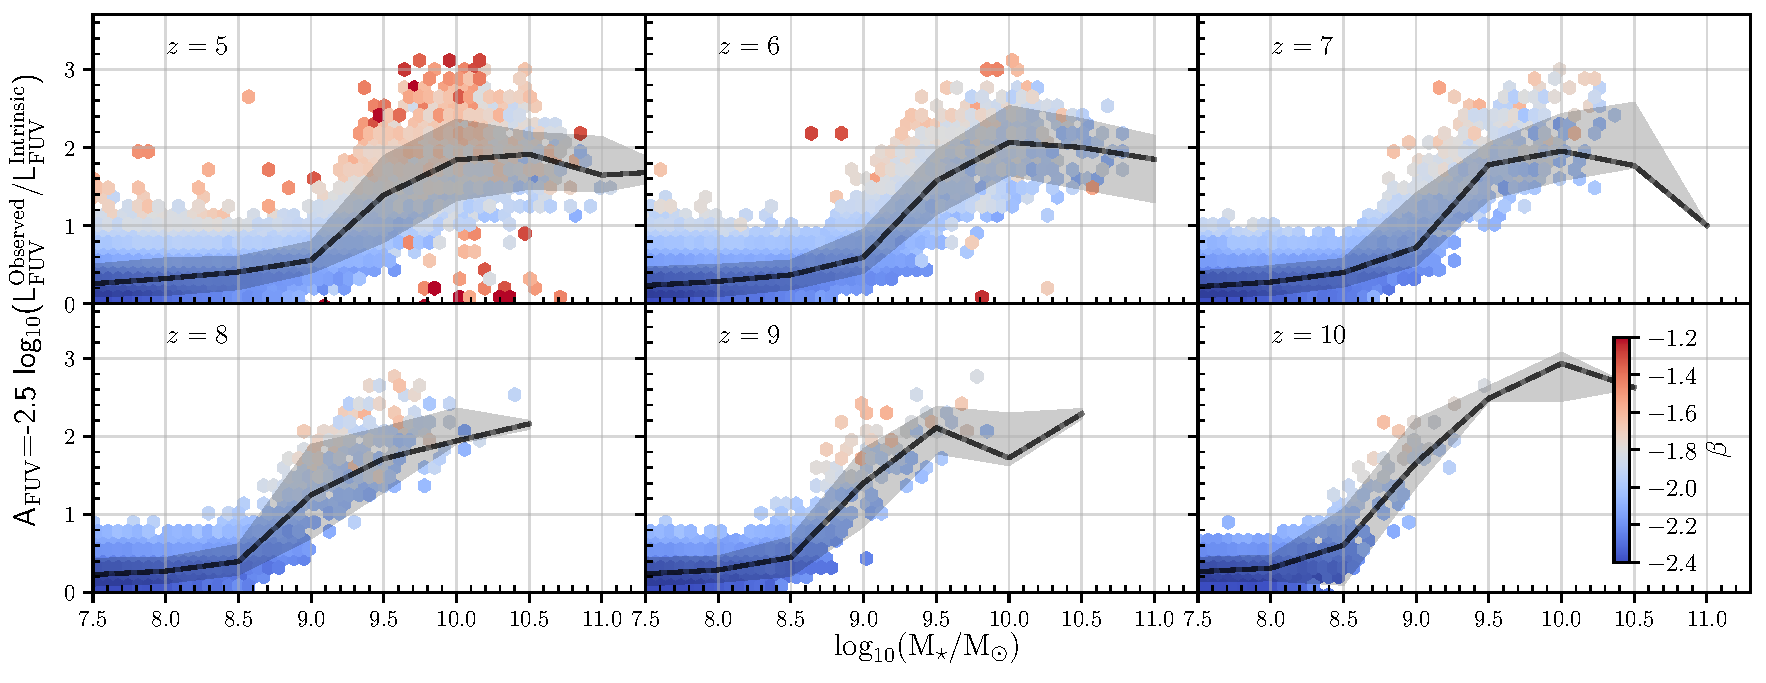
\includegraphics[width=\textwidth]{./figures/att_Mstar_beta_z5_10}
	\caption{The attenuation in the FUV is plotted against the galaxy stellar mass for $z\in[5,10]$. The solid and dashed black line is the weighted median of the sample, with the shaded region indicating the weighted 84 and 16 percentiles. The hexbin denotes the distribution of our sample, coloured by the median $\beta$ value in the hexbin. \label{fig: att_Mstar}} 
\end{figure*} 
For deriving the Schechter and double power-law fit parameters for the UVLF, we calculate the likelihood that the number of observed galaxies in a given magnitude bin is equal to that for an assumed value of the function parameters. This calculation is performed in bins of separation $\Delta M = 0.5$ mag, ranging from from our completeness limit at the faint-end to enclose all our galaxies above this limit. The bin centre and the number density of galaxies per Mag is provided in Table~\ref{tab: LF values}. We use the code \textsf{FitDF}\footnote{\href{https://github.com/flaresimulations/fitDF}{https://github.com/flaresimulations/fitDF}} a Python module for fitting arbitrary distribution functions. \textsf{FitDF} uses \textsf{emcee}, a Python implementation of the affine-invariant ensemble sampler for Markov chain Monte Carlo (MCMC) described in \cite{DFM2013}. The likelihood function is modelled as a Gaussian distribution of the following form
\begin{align}
\mathrm{log}(\mathcal{L}) = - \frac{1}{2} \,  \sum_{i} \,\left[ \frac{ (n_{i,\mathrm{obs}} - n_{i,\mathrm{exp}})^2 }{\sigma_{i}^{2}} \, + \mathrm{log}(\sigma_{i}^{2}) \right] \;\;,
\end{align}
where the subscript $i$ represents the bin of the property being measured, $n_{i,\mathrm{obs}}$ is the number density of galaxies using the composite number density multiplied by the parent box volume, $n_{i,\mathrm{exp}}$ is the expected number density from functional form being used (Schechter or double power-law), and $\sigma_i$ is the error estimate. Using this form, $\sigma$ can be explicitly provided from the resimulated number counts, $\sigma_{i} = n_{i,\mathrm{obs}} / \sqrt{N_{i,\mathrm{obs}}}$, where $N_{i,\mathrm{obs}}$ is the number counts in bin $i$ from the resimulations.

We use flat uniform priors for the parameters in the functional forms. We fix a narrow prior for M$^*$ at $z=9$ for the Schechter functional form. This was done since our fitting function performed poorly in constraining the knee. 

For determining which functional form is better suited at different redshifts we calculated the Bayesian Information Criterion (BIC) value for the best-fit parameters. BIC is a criterion for model selection among a finite set of models. When performing fitting it is possible to increase the likelihood by adding more parameters, but can lead to overfitting. BIC resolves this by implementing a penalty term for the number of parameters in the model; the model with a lower BIC is preferred. A difference of $\sim 20$ in the BIC value is usually taken to be a strong preference for the model with a lower values. 

We also present the relationship between the galaxy stellar mass and the attenuation in the far-UV in Figure~\ref{fig: att_Mstar}. Also shown in the figure is the data points coloured in hexbins of their median UV continuum values ($\beta$) with the solid black line showing the weighted median and the shaded region around it representing the 84 and 16 percentiles of the data. As can be seen from the figure the shape is quite similar to Figure~\ref{fig: att_lfuv} where the attenuation is plotted against the FUV luminosity, the median increases with stelar mass and starts flattening and dropping down afterwards. Also can be seen at $z=5$ is a few of the passive galaxies that have high stellar masses but have lower attenuation.

\section{Calibrating Dust Attenuation}\label{app:calibration}
\begin{figure*}
	\centering
	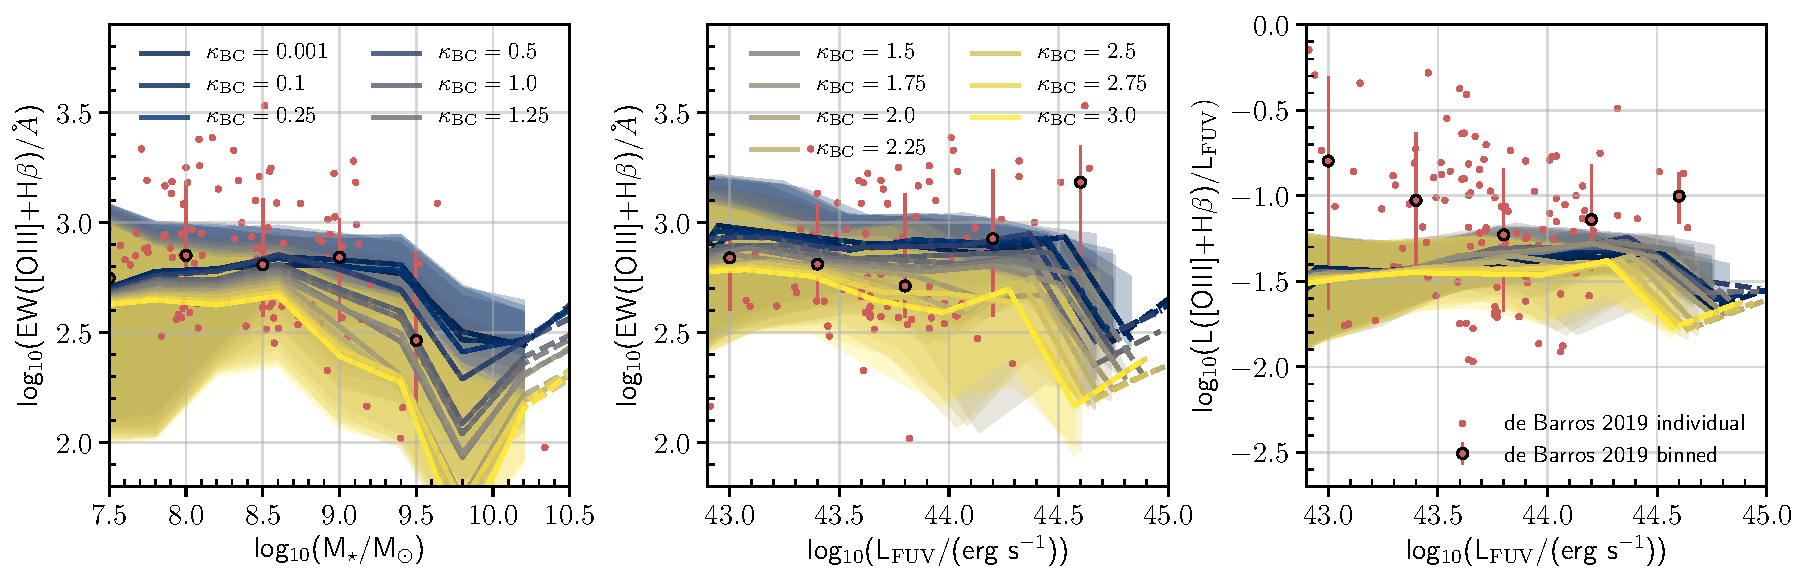
\includegraphics[width=\textwidth]{./figures/App_BC_plot_EW}
	\caption{Same as Figure~\ref{fig: OIII_z7_8}, now showing the line luminosity and equivalent width for different values of $\kappa_{\textrm{BC}}$. The small red circles show the individual measurements from \protect\cite{deBarros19_OIIIHbeta} while the large points denote the median value in bins of stellar mass and far-UV luminosities respectively.\label{fig: line lum diff kappa}}
\end{figure*}
\begin{figure}
	\centering
	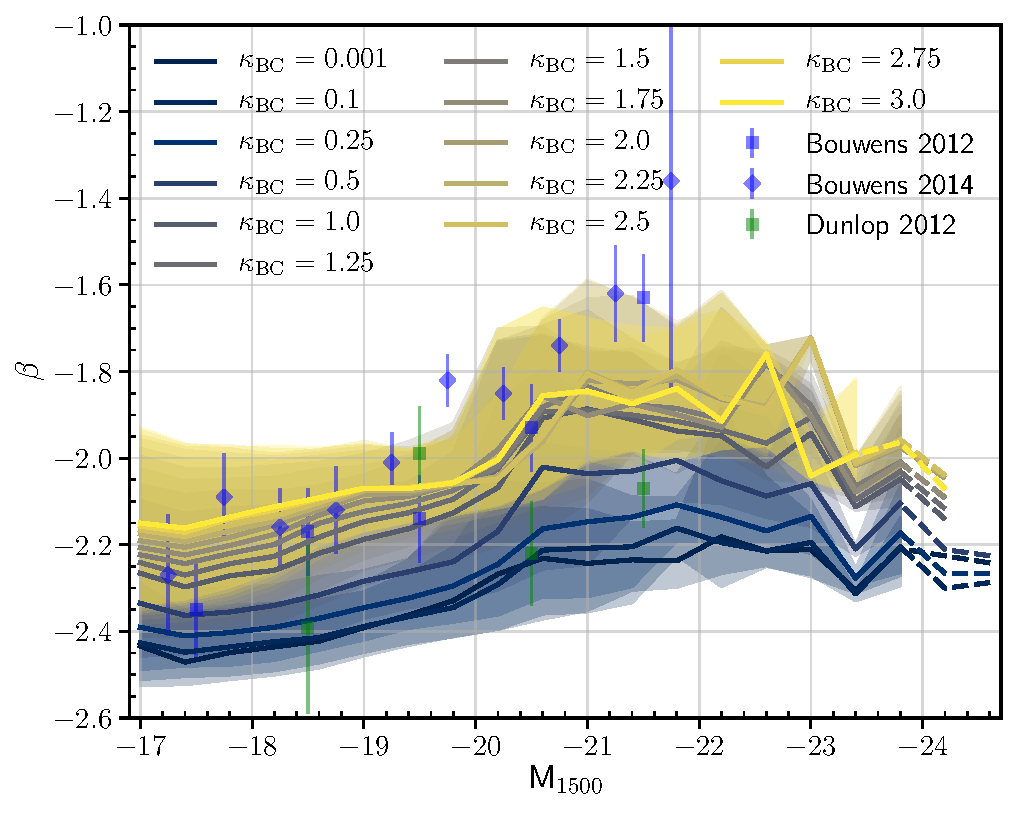
\includegraphics[width=\columnwidth]{./figures/App_BC_plot_beta}
	\caption{UV continuum slope $\beta$ for different values of $\kappa_{\textrm{BC}}$ at $z=5$. Also plotted are the observational data from \protect\cite{Dunlop2012,Bouwens2012b,Bouwens2014a}. \label{fig: beta diff kappa}}
\end{figure}
As noted in \S\ref{sec:modelling.dust} we model the attenuation by dust on a star particle by star particle basis using the integrated line-of-sight surface density of metals as a proxy for dust attenuation. In this simple model we have a two free parameter $\kappa_{\textrm{BC}}$ and $\kappa_{\textrm{ISM}}$ which encapsulates the properties of dust such as the average grain size, shape, composition as well as the dust-to-metal ratio in the birth clouds and in the ISM respectively. To calibrate this model we choose an array of $\kappa_{\textrm{BC}}$ ranging from values of 0 to 3, and then compare our UV LF to observations at $z=5$ from \cite{Bouwens_2015a} to derive a value for $\kappa_{\textrm{ISM}}$. The value for $\kappa_{\textrm{BC}}$ is motivated to get better agreement with the [OIII]$\lambda$4959,5007 line luminosity and equivalent width values from \cite{deBarros19_OIIIHbeta} at $z=8$ (see Figure~\ref{fig: line lum diff kappa}) as well as the UV continuum slope values from literature at $z=5$ (see Figure~\ref{fig: beta diff kappa}). Thus the value is a compromise between choosing a very low value of $\kappa_{\textrm{BC}}$ that agrees with the [OIII] data while a higher value fares better for the UV continuum slope.

\section{Other extinction curves}\label{app:extinction_curves}
\begin{figure}
	\centering
	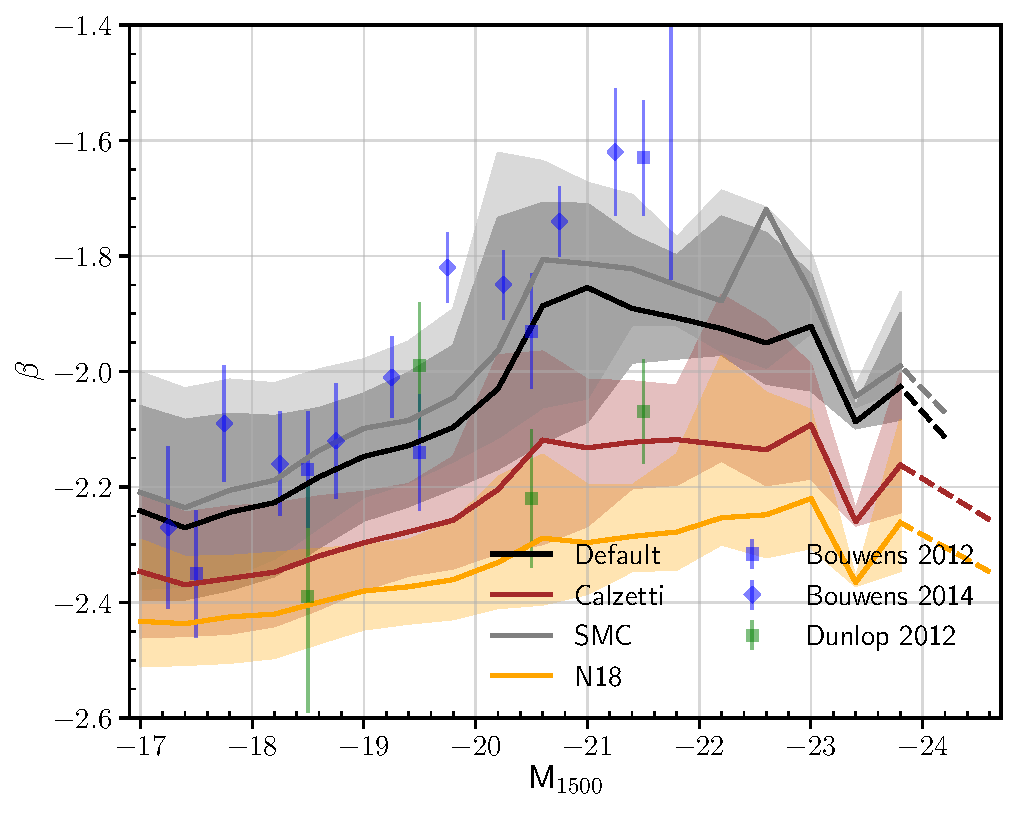
\includegraphics[width=\columnwidth]{./figures/App_beta_Extcurves}
	\caption{UV continuum slope $\beta$ for different extinction curves at $z=5$. Also plotted are the observational data from \protect\cite{Dunlop2012,Bouwens2012b,Bouwens2014a}. \label{fig: ext curves beta}}
\end{figure}
\begin{figure}
	\centering
	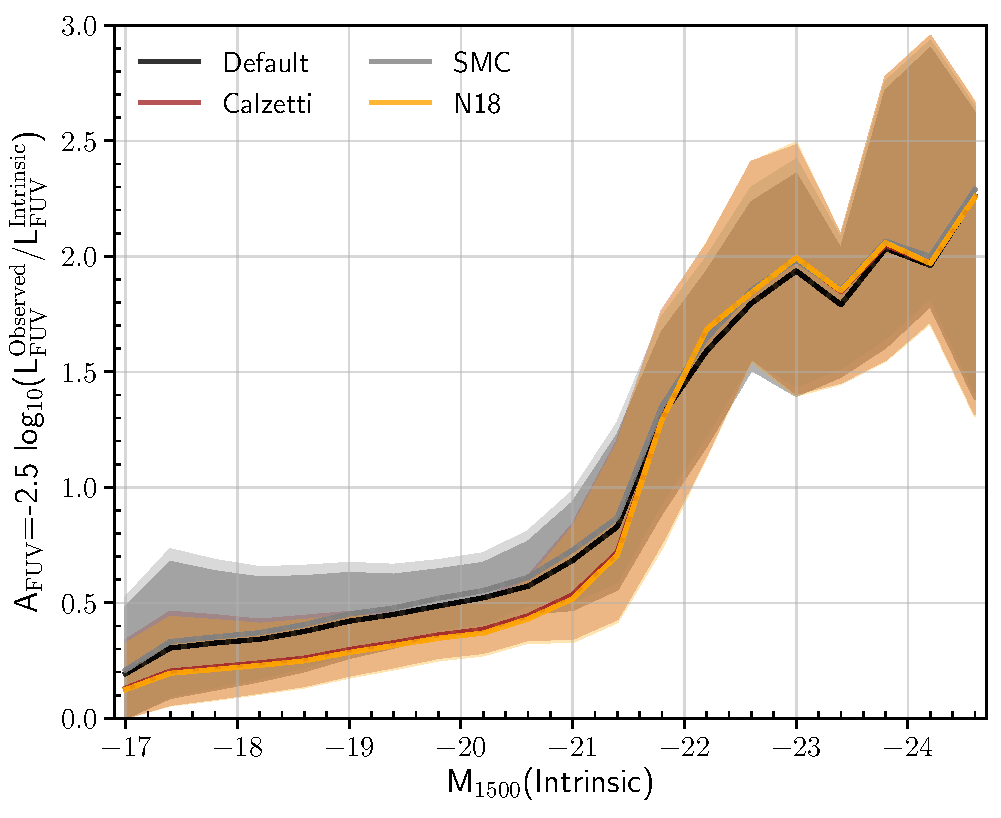
\includegraphics[width=\columnwidth]{./figures/App_Att_Extcurves}
	\caption{Attenuation in far-UV for different extinction curves at $z=5$. Solid lines denotes the weighted median of the sample.\label{fig: ext curves att}}
\end{figure}
\begin{figure*}
	\centering
	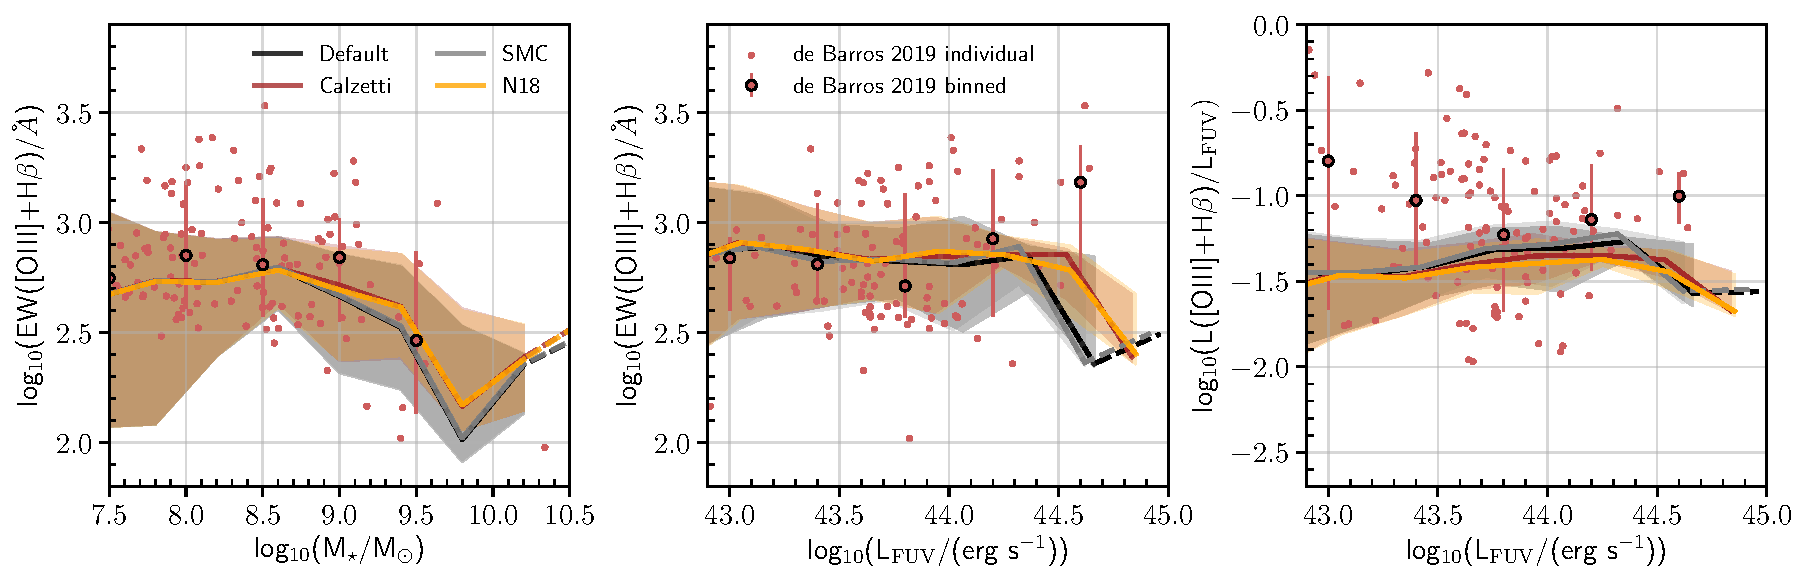
\includegraphics[width=\textwidth]{./figures/App_EW_Extcurves}
	\caption{Same as Figure~\ref{fig: OIII_z7_8}, now showing the line luminosity and equivalent widths for for different extinction curves. The small red circles show the individual measurements from \protect\cite{deBarros19_OIIIHbeta} while the large points denote the median value in bins of stellar mass and far-UV luminosities respectively. \label{fig: ext curves EW}}
\end{figure*}

There has not been any consensus across observational or theoretical studies on the exact nature of the extinction curve in galaxies, since it is closely tied to the properties of the dust grains in galaxies. And this can be inferred better by probing the galaxy SED, and studies have suggested that using a single extinction curve for every galaxy might not be right. In our study we implement a simple extinction curve that is inversely proportional to the wavelength. In this section we will explore how some of the observables presented before changes depending on the chosen extinction curve, namely the Calzetti \citep{Calzetti2000}, Small Magellanic Cloud \citep[SMC, ][]{Pei1992} and the curve used in \cite[][N18 from now on]{Narayanan2018}. 

For this analysis we keep the value of $\kappa_{\textrm{BC}}$ from our default model curve, \ie\, $\kappa_{\textrm{BC}}=1.25$. We then use the method described in Appendix~\ref{app:calibration} to get $\kappa_{\textrm{ISM}}$, obtaining the values of 0.018, 0.0065 and 0.02 for the Calzetti, SMC and N18 curves respectively.

In Figure~\ref{fig: ext curves beta} we present the effect of using different attenuation curves on the UV continuum slope, $\beta$. It can be seen the SMC curve has a higher median for the UV-continuum slope, compared to the default model, a consequence of the SMC curve being steeper than our default value. While for the case of the Calzetti and N18 curves the former has a higher normalization compared to the latter. We also tried increasing the value of $\kappa_{\textrm{BC}}$ for the Calzetti and N18 curves to steepen the relation. We find that the match to the steepness of the observations is difficult to obtain from these curves, implying the \flares\, galaxies prefer a steeper extinction curve similar to the SMC to reproduce the UV-continuum observations.

In Figure~\ref{fig: ext curves EW} we present the effect of using different attenuation curves on the line luminosity and equivalent width relationship of the [OIII]$\lambda$4959,5007 doublet. As can be seen all the curves trace the same space in all the sub-figures. Any minute difference seen happens at higher stellar mass/far-UV luminosity, with the default and SMC curve tracing a higher median than the others.

In Figure~\ref{fig: ext curves att} we present the effect of using different attenuation curves on the attenuation in the far-UV. There is no observed difference in the attenuation in the FUV for any of the curves except at intrinsic M$_{1500}\gtrapprox-21.5$ where the Calzetti and N18 curves produce on average lower attenuation. From our discussion before it is quite clear that despite this the underlying properties vary differently on using these different extinction curves. 

